%QUESTIONS HERE
%<*mytag1>
\begin{questions}[resume,start=\number\value{questionsi}+1,noitemsep,leftmargin=20mm,labelsep=0.1cm]
\item How long does it take for the network to converge to the new route after brining eth2 down?
\end{questions}
%</mytag1>

%<*mytag2>
\begin{questions}[resume,start=\number\value{questionsi}+1,noitemsep,leftmargin=20mm,labelsep=0.1cm]
\item How does the convergence time compare to RIP from Lab 2?
\end{questions}
%</mytag2>

%<*mytag3>
\begin{questions}[resume,start=\number\value{questionsi}+1,noitemsep,leftmargin=20mm,labelsep=0.1cm]
\item How long does it take for the icmp messages to return back to the original route?  How does this time compare to that of Lab 2?
\end{questions}
%</mytag3>

%<*mytag4>
\begin{questions}[resume,start=\number\value{questionsi}+1,noitemsep,leftmargin=20mm,labelsep=0.1cm]
\item Describe what you observe and provide a screenshot.  Anything interesting that you noticed.  Hint:  The route should be somewhat puzzling.
\end{questions}
%</mytag4> 

%<*mytag5>
\begin{questions}[resume*,start=\number\value{questionsi}+1,noitemsep,leftmargin=20mm,labelsep=0.1cm]
\item What do you observe in the Wireshark captures as the reason behind what you discovered in the traceroute?  Provide evidence in the form of screenshots and Wireshark captures.
\end{questions}
%</mytag5> 

%<*mytag6>
\begin{questions}[resume,start=\number\value{questionsi}+1,noitemsep,leftmargin=20mm,labelsep=0.1cm]
\item What commands did you use to redistribute static routes in RIP? How did we redistribute the static routes using Babel?
\end{questions}
%</mytag6> 

%<*mytag7>
\begin{questions}[resume*,start=\number\value{questionsi}+1,noitemsep,leftmargin=20mm,labelsep=0.1cm]
\item Referring to your answer to the previous question about Babel, does this command only redistribute static routes?
\end{questions}
%</mytag7>

%<*mytag8>
\begin{questions}[resume,start=\number\value{questionsi}+1,noitemsep,leftmargin=20mm,labelsep=0.1cm]
\item What protocol is used by Babel that is not used by RIPv2 by default? What protocol do they both use?
\end{questions}
%</mytag8>

%<*mytag9>
\begin{questions}[resume,start=\number\value{questionsi}+1,noitemsep,leftmargin=20mm,labelsep=0.1cm]
\item 
\item
\end{questions}
%</mytag9>

%LISTS HERE

%<*mytag10>
\begin{enumerate}[noitemsep,label=$\circ$,leftmargin=17mm,labelsep=0.5cm]
\item
\item
\end{enumerate}
%</mytag10>

%<*mytag11>
\begin{enumerate}[noitemsep,leftmargin=10mm,labelsep=0.1cm]
\item Test item
\item
\end{enumerate}
%</mytag11>


%COMMANDS HERE
%<*mytag12>
\begin{enumerate}[noitemsep,leftmargin=10mm,labelsep=0.1cm]
\item [] \textbf{}  
\end{enumerate}
%</mytag12>

%<*mytag13>
\begin{enumerate}[noitemsep,leftmargin=10mm,labelsep=0.1cm]
\item [] \textbf{dpkg -s gcc bison flex}
\end{enumerate}
%</mytag13>
%<*mytag14>
\begin{enumerate}[noitemsep,label=$\circ$,leftmargin=17mm,labelsep=0.5cm]
\item [] \textbf{./configure -help}
\end{enumerate}
%</mytag14>
%<*mytag15>
\begin{enumerate}[noitemsep,leftmargin=10mm,labelsep=0.1cm]
\item [] \textbf{./configure --enable-acls --enable-uenable && make install}
\end{enumerate}
%</mytag15>
%<*mytag16>
\begin{enumerate}[noitemsep,leftmargin=10mm,labelsep=0.1cm]
\item [] \textbf{tac\_pwd}
\end{enumerate}
%</mytag16>
%<*mytag17>
\begin{enumerate}[noitemsep,leftmargin=10mm,labelsep=0.1cm]
\item [] \textbf{Password to be encrypted: \<your password here\>}
\end{enumerate}
%</mytag17>
%<*mytag18>
\begin{enumerate}[noitemsep,leftmargin=10mm,labelsep=0.1cm]
\item [] \textbf{touch /etc/default/tac\textunderscore plus}
\end{enumerate}
%</mytag18>
%<*mytag19>
\begin{enumerate}[noitemsep,leftmargin=10mm,labelsep=0.1cm]
\item [] \textbf{chmod 755 /etc/default/tac\textunderscore plus}
\end{enumerate}
%</mytag19>
%<*mytag20>
\begin{enumerate}[noitemsep,leftmargin=10mm,labelsep=0.1cm]
\item [] \textbf{nano /etc/default/tac\textunderscore plus}
\end{enumerate}
%</mytag20>
%<*mytag21>
\begin{enumerate}[noitemsep,leftmargin=10mm,labelsep=0.1cm]
\item [] \textbf{/etc/init.d/tac\textunderscore plus start}
\end{enumerate}
%</mytag21>
%<*mytag22>
\begin{enumerate}[noitemsep,leftmargin=10mm,labelsep=0.1cm]
\item [] \textbf{ps aux | grep tac\textunderscore plus} 
\end{enumerate}
%</mytag22>
%<*mytag23>
\begin{enumerate}[noitemsep,leftmargin=10mm,labelsep=0.1cm]
\item [] \textbf{netstat -an | grep :49}
\end{enumerate}
%</mytag23>
%<*mytag24>
\begin{enumerate}[noitemsep,leftmargin=10mm,labelsep=0.1cm]
\item [] \textbf{services}
\end{enumerate}
%</mytag24>
%<*mytag25>
\begin{enumerate}[noitemsep,leftmargin=10mm,labelsep=0.1cm]
\item [] \textbf{vulns}
\end{enumerate}
%</mytag25>
%<*mytag26>
\begin{enumerate}[noitemsep,leftmargin=10mm,labelsep=0.1cm]
\item [] \textbf{db\_import $<$name of the Nessus scan file including path$>$}
\end{enumerate}
%</mytag26>
%<*mytag27>
\begin{enumerate}[noitemsep,leftmargin=10mm,labelsep=0.1cm]
\item [] \textbf{vulns}
\end{enumerate}
%</mytag27>

%<*mytag28>
\begin{enumerate}[noitemsep,label=$\circ$,leftmargin=14mm,labelsep=0.5cm]
\item
\end{enumerate}
%</mytag28>


%GRAPHICS HERE


%<*mtag1>
\begin{figure}[H]
\centering
\captionsetup{width=.8\linewidth}
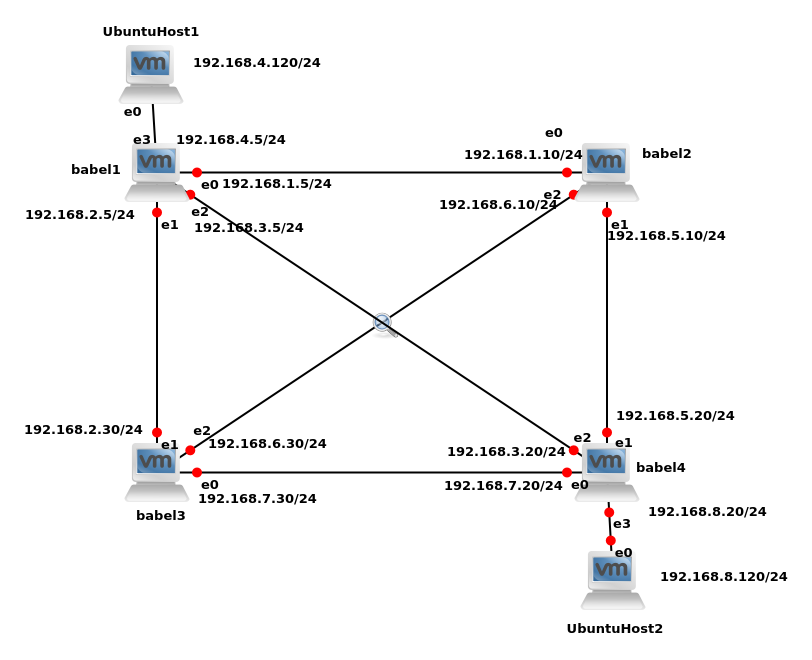
\includegraphics[scale=0.60]{img/EX2NetDiagram.png}
\caption{Network Diagram for Exercise 2}
\label{fig:ex2Net}
\centering
\end{figure}
%</mtag1>


%<*mtag2>
\begin{figure}[H]
\centering
\captionsetup{width=.8\linewidth}
\includegraphics[scale=0.9]{img/.png}
\caption{}
\label{fig:2}
\centering
\end{figure}
%</mtag2>

%<*mtag3>
\begin{figure}[H]
\centering
\captionsetup{width=.8\linewidth}
\includegraphics[scale=0.9]{img/.png}
\caption{}
\label{fig:3}
\centering
\end{figure}
%</mtag3>